\section{Resultados}

Para a análise dos dados dos resultados, considere a rede didática de 45 nós com os seguintes parâmetros:

\begin{table}[H]\footnotesize
    \begin{minipage}{.5\linewidth}
        \caption{Parâmetros de impedância e corrente máxima para o conjunto de circuitos da rede didática de 45 nós}
        \centering
        \begin{table}[H]
    \label{tab:impedancia}
    \caption{Parâmetros de impedância e corrente máxima para o conjunto de circuitos da rede didática de 45 nós}
    \begin{minipage}{.5\linewidth}
        \centering
        \begin{tabular}{|c|c|c|c|c|}
        \hline
        $b_\text{part}$ & $b_\text{cheg}$& R [$\Omega$]  & X [$\Omega$] & Imax [A]\\ \hline
         2 &  3 & 0.0922 & 0.0470 & 200\\ \hline
         3 &  4 & 0.4930 & 0.2511 & 200\\ \hline
         4 &  5 & 0.3660 & 0.1864 & 200\\ \hline
         5 &  6 & 0.3811 & 0.1941 & 200\\ \hline
         6 &  7 & 0.8190 & 0.7070 & 200\\ \hline
         7 &  8 & 0.1872 & 0.6188 & 200\\ \hline
         9 & 10 & 0.7114 & 0.2351 & 200\\ \hline
        10 & 11 & 10.300 & 0.7400 & 200\\ \hline
        11 & 13 & 10.440 & 0.7400 & 200\\ \hline
        13 & 14 & 0.1966 & 0.0650 & 200\\ \hline
        14 & 15 & 0.3744 & 0.1238 & 200\\ \hline
        15 & 16 & 14.680 & 11.550 & 200\\ \hline
        17 & 18 & 0.5416 & 0.7129 & 200\\ \hline
        18 & 19 & 0.5910 & 0.5260 & 200\\ \hline
        19 & 20 & 0.7463 & 0.5450 & 200\\ \hline
        20 & 21 & 12.890 & 17.210 & 200\\ \hline
        21 & 22 & 0.7320 & 0.5740 & 200\\ \hline
         3 & 23 & 0.1640 & 0.1565 & 200\\ \hline        
        \end{tabular}
        
    \end{minipage}%
    \begin{minipage}{.5\linewidth}
        \centering
        \begin{tabular}{|c|c|c|c|c|}
        \hline
        $b_\text{part}$ & $b_\text{cheg}$& R [$\Omega$]  & X [$\Omega$] & Imax [A]\\ \hline    
        24 & 25 & 15.042 & 13.554 & 200\\ \hline
        25 & 26 & 0.4095 & 0.4784 & 200\\ \hline
        26 & 27 & 0.7089 & 0.9373 & 200\\ \hline
         4 & 30 & 0.4512 & 0.3083 & 200\\ \hline
        31 & 32 & 0.8980 & 0.7091 & 200\\ \hline
        32 & 33 & 0.8960 & 0.7011 & 200\\ \hline
         7 & 35 & 0.2030 & 0.1034 & 200\\ \hline
        36 & 37 & 0.2842 & 0.1447 & 200\\ \hline
        37 & 38 & 10.590 & 0.9337 & 200\\ \hline
        38 & 39 & 0.8042 & 0.7006 & 200\\ \hline
        39 & 40 & 0.5075 & 0.2585 & 200\\ \hline
        41 & 42 & 0.9744 & 0.9630 & 200\\ \hline
        42 & 43 & 0.3105 & 0.3619 & 200\\ \hline
        43 & 44 & 0.3410 & 0.5302 & 200\\ \hline
        10 & 28 & 20.000 & 20.000 & 200\\ \hline
        12 & 19 & 20.000 & 20.000 & 200\\ \hline
        18 & 29 & 20.000 & 20.000 & 200\\ \hline
        22 & 45 & 0.5000 & 0.5000 & 200\\ \hline
        34 & 39 & 0.5000 & 0.5000 & 200\\ \hline
        \end{tabular}
    \end{minipage} 
\end{table}
    \end{minipage}%
    \begin{minipage}{.5\linewidth}
        \centering
        \caption{Potência ativa e reativa de demanda para cada nó da rede didática de 45 nós}
        \begin{table}[H]
    \label{tab:demanda}
    \caption{Potência ativa e reativa de demanda para cada nó da rede didática de 45 nós}
    
    \begin{minipage}{.5\linewidth}
        \centering

        \begin{tabular}{|c|c|c|c|}
            \hline
            $\Omega_b$ & $T_b$ & $P_D$ [kW] & $Q_D$ [kVar]\\ \hline
            1  &  1 &  0.001 &  0.001\\ \hline 
            2  &  0 &  0.001 &  0.001\\ \hline
            3  &  0 &   30.0 &   10.0\\ \hline
            4  &  0 &   30.0 &   10.0\\ \hline
            5  &  0 &   40.0 &   15.0\\ \hline
            6  &  0 &   20.0 &   10.0\\ \hline
            7  &  0 &   20.0 &    5.0\\ \hline
            8  &  0 &   60.0 &   30.0\\ \hline
            9  &  0 &  0.001 &  0.001\\ \hline
            10 &  0 &   60.0 &   30.0\\ \hline
            11 &  0 &   20.0 &    5.0\\ \hline
            12 &  0 &  0.001 &  0.001\\ \hline
            13 &  0 &   20.0 &    5.0\\ \hline
            14 &  0 &   15.0 &   10.0\\ \hline
            15 &  0 &   20.0 &   10.0\\ \hline
            16 &  0 &  0.001 &  0.001\\ \hline
            17 &  0 &   20.0 &   10.0\\ \hline
            18 &  0 &   40.0 &   15.0\\ \hline
            19 &  0 &   20.0 &    5.0\\ \hline
            20 &  0 &   20.0 &    5.0\\ \hline
            21 &  0 &   20.0 &    5.0\\ \hline
            22 &  0 &   30.0 &   10.0\\ \hline
            23 &  0 &  0.001 &  0.001\\ \hline
                 
        \end{tabular}
        
    \end{minipage}%
    \begin{minipage}{.5\linewidth}
        \centering
         \begin{tabular}{|c|c|c|c|} 
            \hline
            $\Omega_b$ & $T_b$ & $P_D$ [kW] & $Q_D$ [kVar]\\ \hline
            24 &  0 &   30.0 &   10.0\\ \hline
            25 &  0 &   30.0 &   10.0\\ \hline
            26 &  0 &   30.0 &   10.0\\ \hline
            27 &  0 &   30.0 &   10.0\\ \hline
            28 &  0 &  0.001 &  0.001\\ \hline
            29 &  0 &  0.001 &  0.001\\ \hline
            30 &  0 &   30.0 &   10.0\\ \hline
            31 &  0 &  0.001 &  0.001\\ \hline
            32 &  0 &  140.0 &   60.0\\ \hline
            33 &  0 &  140.0 &   60.0\\ \hline
            34 &  0 &  0.001 &  0.001\\ \hline
            35 &  0 &   20.0 &    5.0\\ \hline
            36 &  0 &  0.001 &  0.001\\ \hline
            37 &  0 &   20.0 &    5.0\\ \hline
            38 &  0 &   20.0 &    5.0\\ \hline
            39 &  0 &   40.0 &   15.0\\ \hline
            40 &  0 &   60.0 &   30.0\\ \hline
            41 &  0 &  0.001 &  0.001\\ \hline
            42 &  0 &   50.0 &   10.0\\ \hline
            43 &  0 &   70.0 &   30.0\\ \hline
            44 &  0 &   20.0 &    5.0\\ \hline
            45 &  0 &  0.001 &  0.001\\ \hline

            
            \end{tabular}
    \end{minipage} 
\end{table}
    \end{minipage} 
\end{table}

\begin{table}[H]
    \centering
    \caption{Estado das chaves antes da otimização}
    \label{tab:est_chave_atual}
    \begin{tabular}{|c|c|c|c|}
        \hline
        \multicolumn{2}{|c|}{$\Omega_{ch}$} & $w_{ij}$ & $I_{maxch}$ [A]\\ \hline
         1 &   2 &  1 &   500\\ \hline
         8 &   9 &  1 &   500\\ \hline
        11 &  12 &  0 &   500\\ \hline
        16 &  17 &  1 &   500\\ \hline
        23 &  24 &  1 &   500\\ \hline
        26 &  28 &  0 &   500\\ \hline
        27 &  29 &  0 &   500\\ \hline
        30 &  31 &  1 &   500\\ \hline
        33 &  34 &  0 &   500\\ \hline
        35 &  36 &  1 &   500\\ \hline
        40 &  41 &  1 &   500\\ \hline
        44 &  45 &  0 &   500\\ \hline
    \end{tabular}
\end{table}

%Identificar o perfil de tensão ao longo da rede de distribuição


\begin{figure}[H]
    \centering
    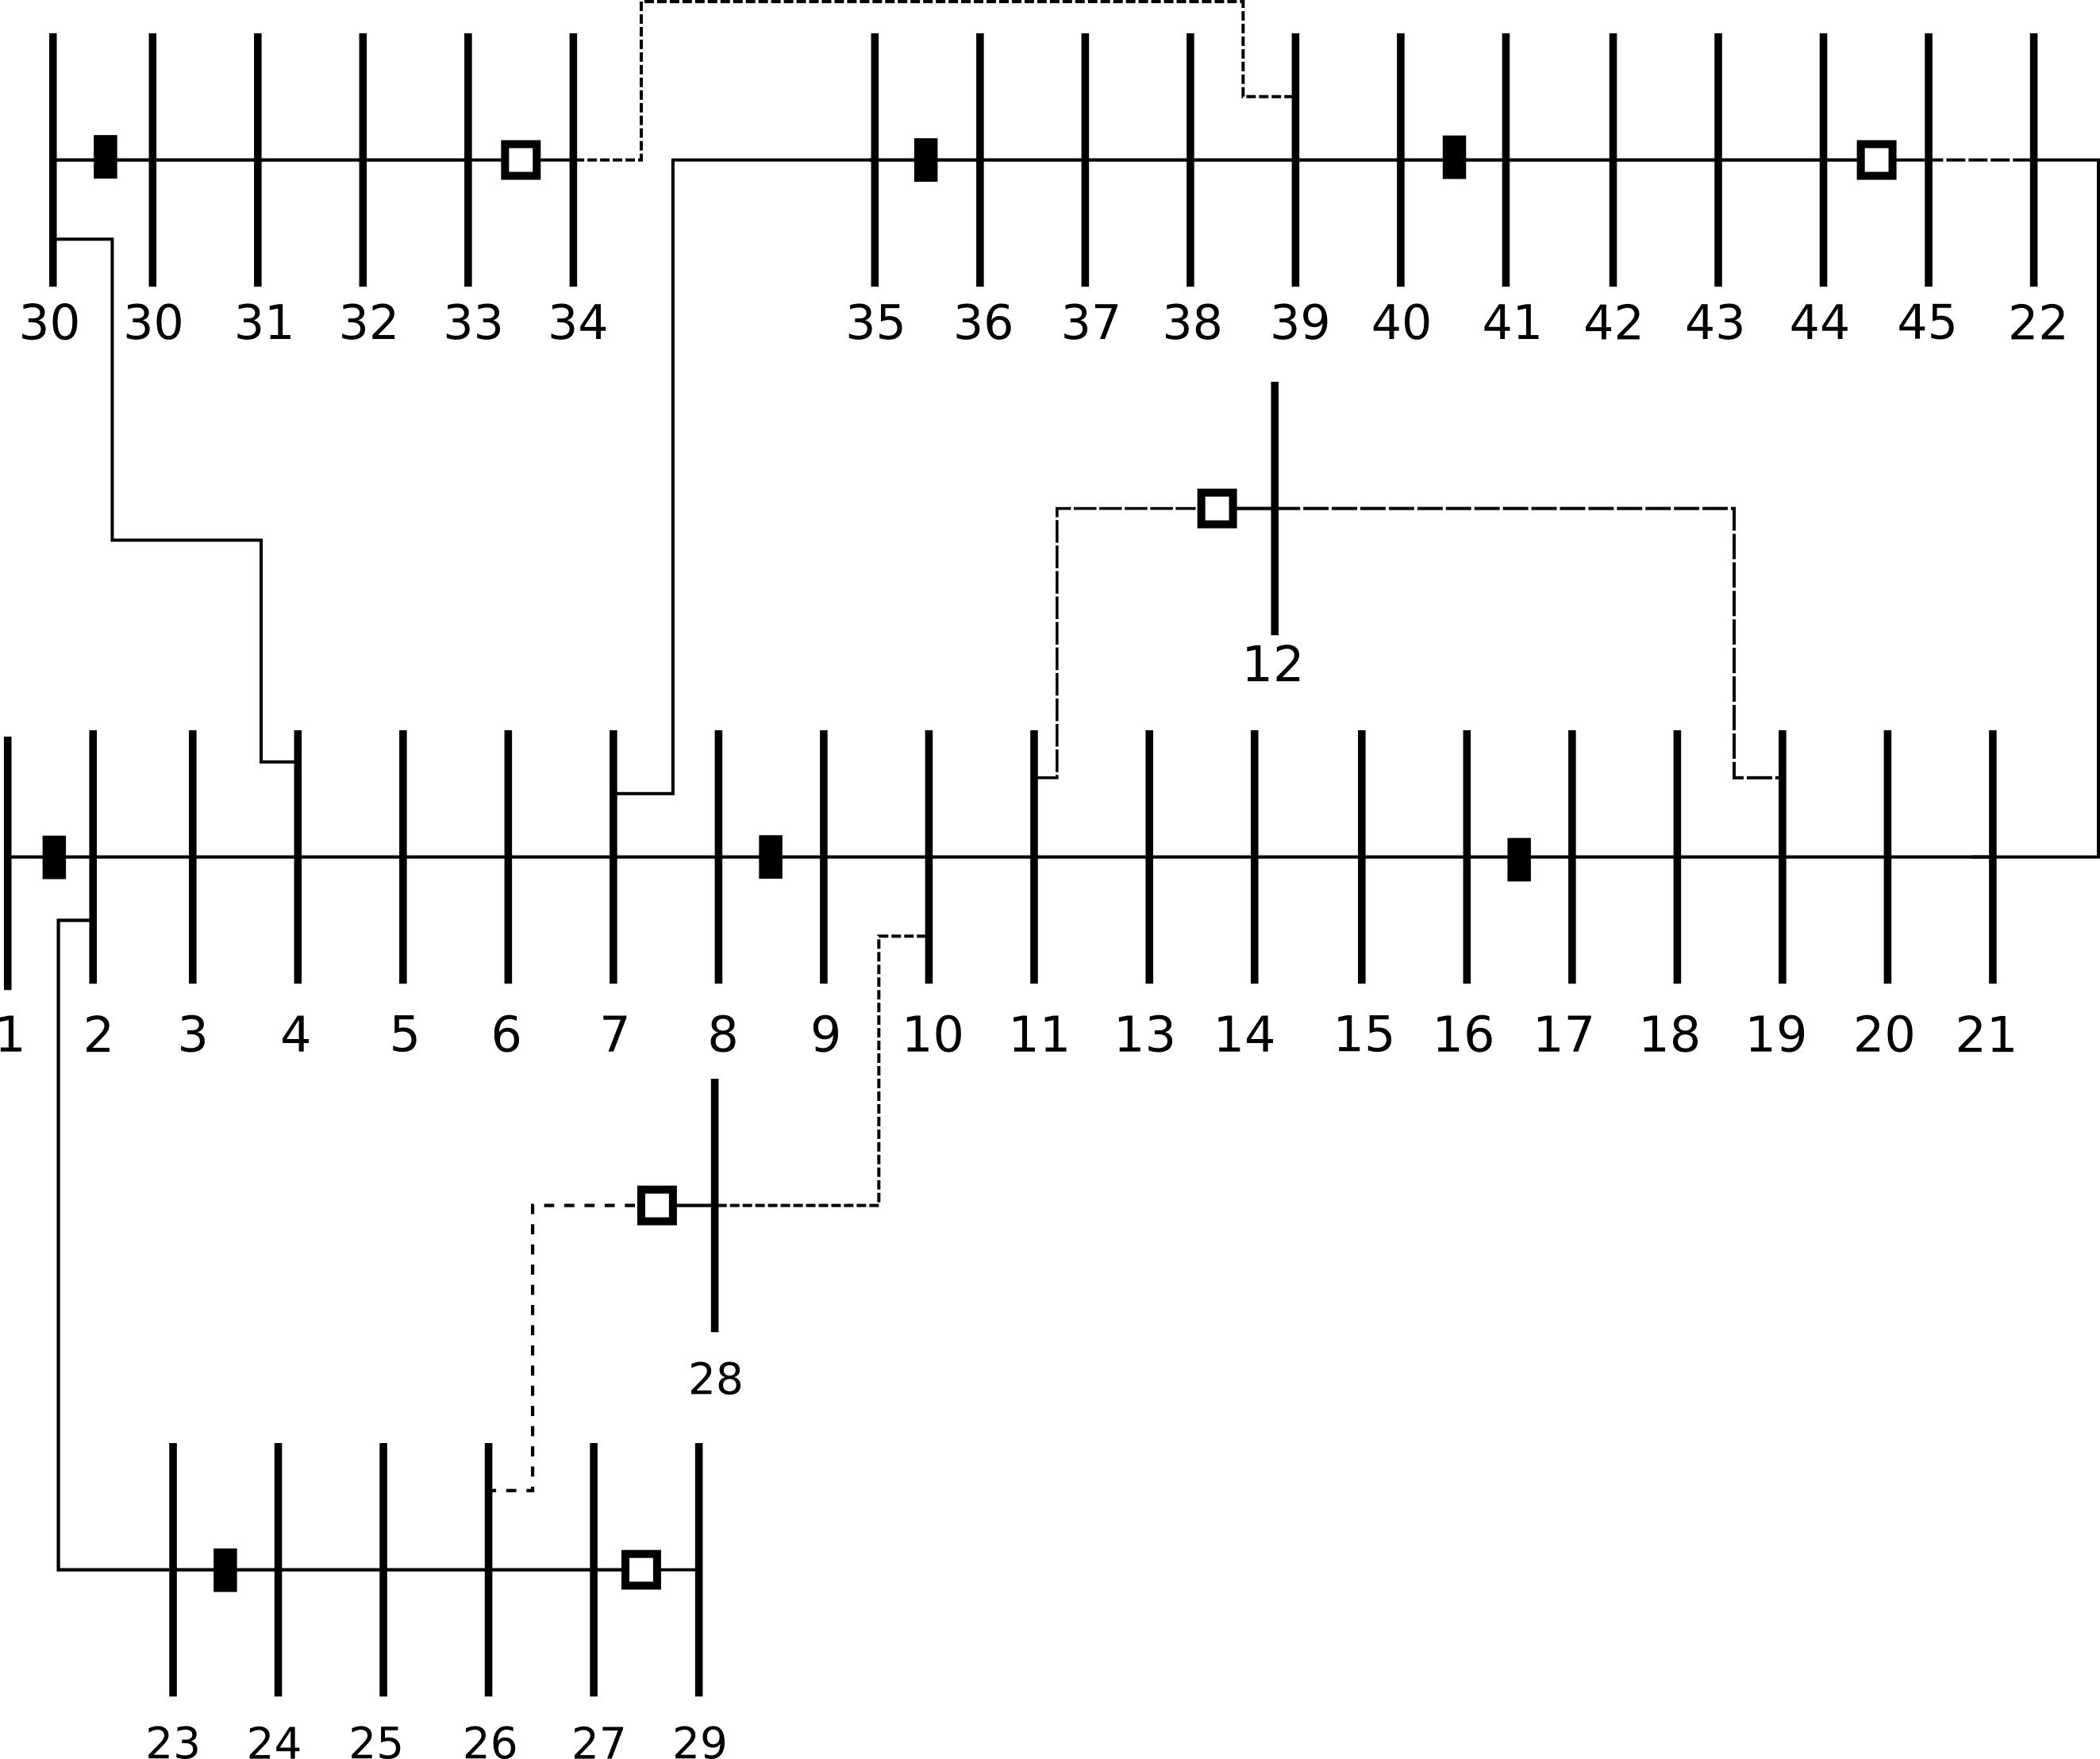
\includegraphics[width=\textwidth]{01_img/Diagrama_inicial.png}
    \caption{Estado inicial da rede de distribuição com alimentador no nó 1}  
    \label{fig:rede_inic}
\end{figure}

\begin{table}[H]\footnotesize
    \caption{Fluxo de potência reativa entre nós no sistema de 45 nós atual}
    \label{tab:fluxo_kW_atual}
    \begin{minipage}{.5\linewidth}
        \centering
        \begin{tabular}{|c|c|c|}
            \hline
            \multicolumn{2}{|c|}{$\Omega_l$} & $P_{ij}$ [kW]  \\ \hline
             2 &   3 & 1293.97\\ \hline
             3 &   4 & 1131.21\\ \hline
             4 &   5 &  785.09\\ \hline
             5 &   6 &  741.52\\ \hline
             6 &   7 &  714.26\\ \hline
             7 &   8 &  377.37\\ \hline
             9 &  10 &  316.12\\ \hline
            10 &  11 &  244.39\\ \hline
            11 &  13 &  214.30\\ \hline
            13 &  14 &  194.15\\ \hline
            14 &  15 &  178.89\\ \hline
            15 &  16 &  151.18\\ \hline
            17 &  18 &  130.97\\ \hline
            18 &  19 &   90.86\\ \hline
            19 &  20 &   70.78\\ \hline
            20 &  21 &   50.02\\ \hline
            21 &  22 &   30.00\\ \hline
             3 &  23 &  122.09\\ \hline
        \end{tabular}
    \end{minipage}%
    \begin{minipage}{.5\linewidth}
        \centering
        \begin{tabular}{|c|c|c|}
            \hline
            \multicolumn{2}{|c|}{$\Omega_l$} & $P_{ij}$ [kW]  \\ 
            \hline
            24 &  25 &   90.04\\ \hline
            25 &  26 &   60.01\\ \hline
            26 &  27 &   30.00\\ \hline
             4 &  30 &  311.55\\ \hline
            31 &  32 &  280.31\\ \hline
            32 &  33 &  140.00\\ \hline
             7 &  35 &  316.06\\ \hline
            36 &  37 &  295.63\\ \hline
            37 &  38 &  261.72\\ \hline
            38 &  39 &  240.82\\ \hline
            39 &  40 &  200.42\\ \hline
            41 &  42 &  140.05\\ \hline
            42 &  43 &   90.00\\ \hline
            43 &  44 &   20.00\\ \hline
            10 &  28 &    0.00\\ \hline
            12 &  19 &   -0.00\\ \hline
            18 &  29 &    0.00\\ \hline
            22 &  45 &    0.00\\ \hline
            34 &  39 &   -0.00\\ \hline        
        \end{tabular}
    \end{minipage} 
\end{table}


  



\begin{table}[H]\footnotesize
    \caption{Fluxo de potência reativa entre nós no sistema de 45 nós atual}
    \label{tab:fluxo_kvar_atual}
    \begin{minipage}{.5\linewidth}
        \centering
        \begin{tabular}{|c|c|c|}
            \hline
            \multicolumn{2}{|c|}{$\Omega_l$} & $Q_{ij}$ [kVar]  \\ \hline
             2  &  3 &  498.36\\ \hline
             3  &  4 &  441.02\\ \hline
             4  &  5 &  297.33\\ \hline
             5  &  6 &  280.51\\ \hline
             6  &  7 &  264.25\\ \hline
             7  &  8 &  149.64\\ \hline
             9  & 10 &  119.23\\ \hline
            10  & 11 &   88.38\\ \hline
            11  & 13 &   82.67\\ \hline
            13  & 14 &   77.62\\ \hline
            14  & 15 &   67.53\\ \hline
            15  & 16 &   51.47\\ \hline
            17  & 18 &   41.19\\ \hline
            18  & 19 &   26.09\\ \hline
            19  & 20 &   21.03\\ \hline
            20  & 21 &   15.01\\ \hline
            21  & 22 &   10.00\\ \hline
             3  & 23 &   41.89\\ \hline
        \end{tabular}
    \end{minipage}%
    \begin{minipage}{.5\linewidth}
        \centering
        \begin{tabular}{|c|c|c|}
            \hline
            \multicolumn{2}{|c|}{$\Omega_l$} & $Q_{ij}$ [kVAr]  \\ 
            \hline
            24 &  25 &    30.04\\ \hline
            25 &  26 &    20.01\\ \hline
            26 &  27 &    10.00\\ \hline
             4 &  30 &   131.22\\ \hline
            31 &  32 &   120.24\\ \hline
            32 &  33 &    60.00\\ \hline
             7 &  35 &   107.86\\ \hline
            36 &  37 &   102.64\\ \hline
            37 &  38 &    96.42\\ \hline
            38 &  39 &    90.63\\ \hline
            39 &  40 &    75.42\\ \hline
            41 &  42 &    45.06\\ \hline
            42 &  43 &    35.00\\ \hline
            43 &  44 &     5.00\\ \hline
            10 &  28 &     0.00\\ \hline
            12 &  19 &    -0.00\\ \hline
            18 &  29 &     0.00\\ \hline
            22 &  45 &     0.00\\ \hline
            34 &  39 &    -0.00\\ \hline
        \end{tabular}
    \end{minipage} 
\end{table}




\begin{table}[H]
    \centering
    \label{tab:pot_chav_atual}
    \caption{Fluxo de potência nas chaves de interconexão do sistema atual}
     \subfloat[Fluxo de potência ativa]{
         \centering
         \begin{tabular}{|c|c|c|}
            \hline
            \multicolumn{2}{|c|}{$\Omega_l$} & $P_{ij}$ [kVAr]  \\ 
            \hline
               1 &   2 & 1296.52\\ \hline
               8 &   9 &  317.37\\ \hline
              11 &  12 &    0.00\\ \hline
              16 &  17 &  151.18\\ \hline
              23 &  24 &  122.09\\ \hline
              26 &  28 &    0.00\\ \hline
              27 &  29 &    0.00\\ \hline
              30 &  31 &  281.55\\ \hline
              33 &  34 &    0.00\\ \hline
              35 &  36 &  296.06\\ \hline
              40 &  41 &  140.42\\ \hline
              44 &  45 &    0.00\\ \hline     
         \end{tabular}
     }
     \hspace{3cm} %altera o espaçamento entre as tabelas
     \subfloat[Fluxo de potência reativa]{
         \centering
         \begin{tabular}{|c|c|c|}
            \hline
            \multicolumn{2}{|c|}{$\Omega_l$} & $Q_{ij}$ [kVAr]  \\ 
            \hline
               1 &   2 &  499.66\\ \hline
               8 &   9 &  119.64\\ \hline
              11 &  12 &    0.00\\ \hline
              16 &  17 &   51.47\\ \hline
              23 &  24 &   41.89\\ \hline
              26 &  28 &    0.00\\ \hline
              27 &  29 &    0.00\\ \hline
              30 &  31 &  121.22\\ \hline
              33 &  34 &    0.00\\ \hline
              35 &  36 &  102.86\\ \hline
              40 &  41 &   45.42\\ \hline
              44 &  45 &    0.00\\ \hline
        \end{tabular}
     }
\end{table}

\begin{figure}[H]
    \centering
    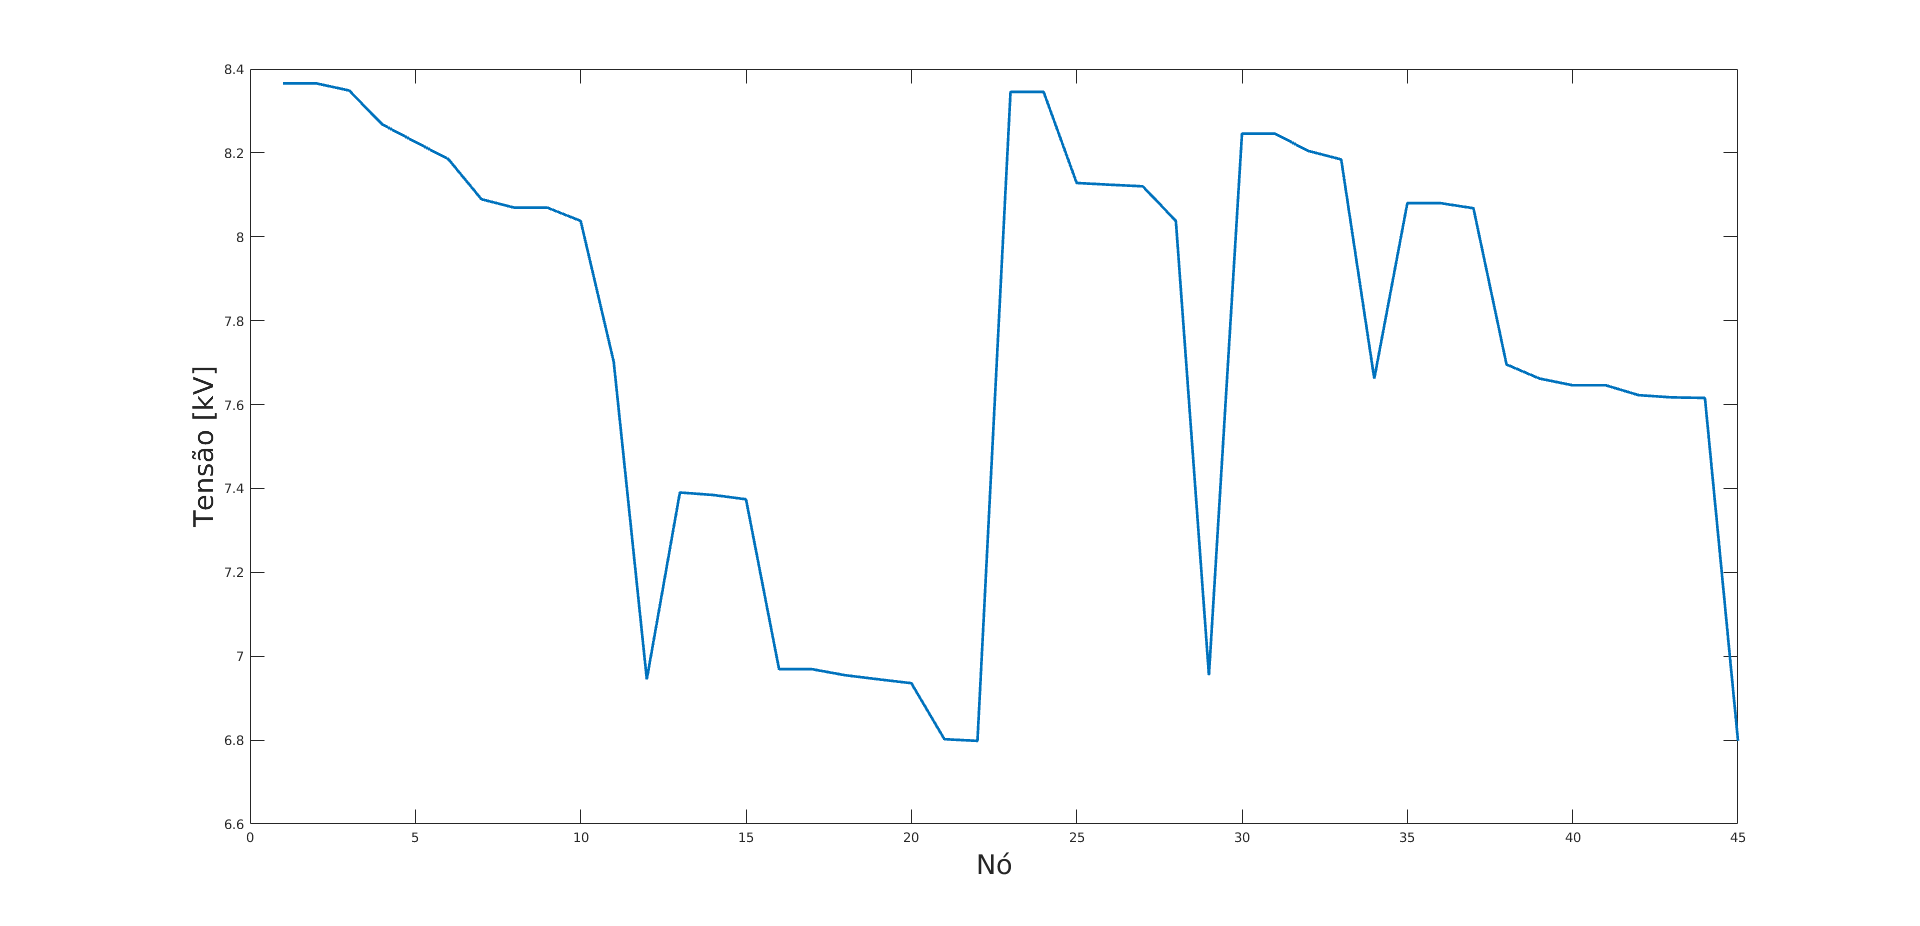
\includegraphics[width=\textwidth]{01_img/Perfil_tensao_atual.png}
    \caption{Perfil da tensão da rede atual}
    \label{fig:voltages_atual}
\end{figure}






%rede já otimizada

\begin{table}[H]
    \centering
    \caption{Estado das chaves após da otimização}
    \label{tab:est_chave_otim}
    \begin{tabular}{|c|c|c|c|}
        \hline
        \multicolumn{2}{|c|}{$\Omega_{ch}$} & $w_{ij}$\\ \hline
         1 &   2    & 1\\ \hline
         8 &   9    & 1\\ \hline
        11 &  12    & 0\\ \hline
        16 &  17    & 0\\ \hline
        23 &  24    & 1\\ \hline
        26 &  28    & 0\\ \hline
        27 &  29    & 0\\ \hline
        30 &  31    & 1\\ \hline
        33 &  34    & 1\\ \hline
        35 &  36    & 0\\ \hline
        40 &  41    & 1\\ \hline
        44 &  45    & 1\\ \hline
    \end{tabular}
\end{table}

\begin{figure}[H]
    \centering
    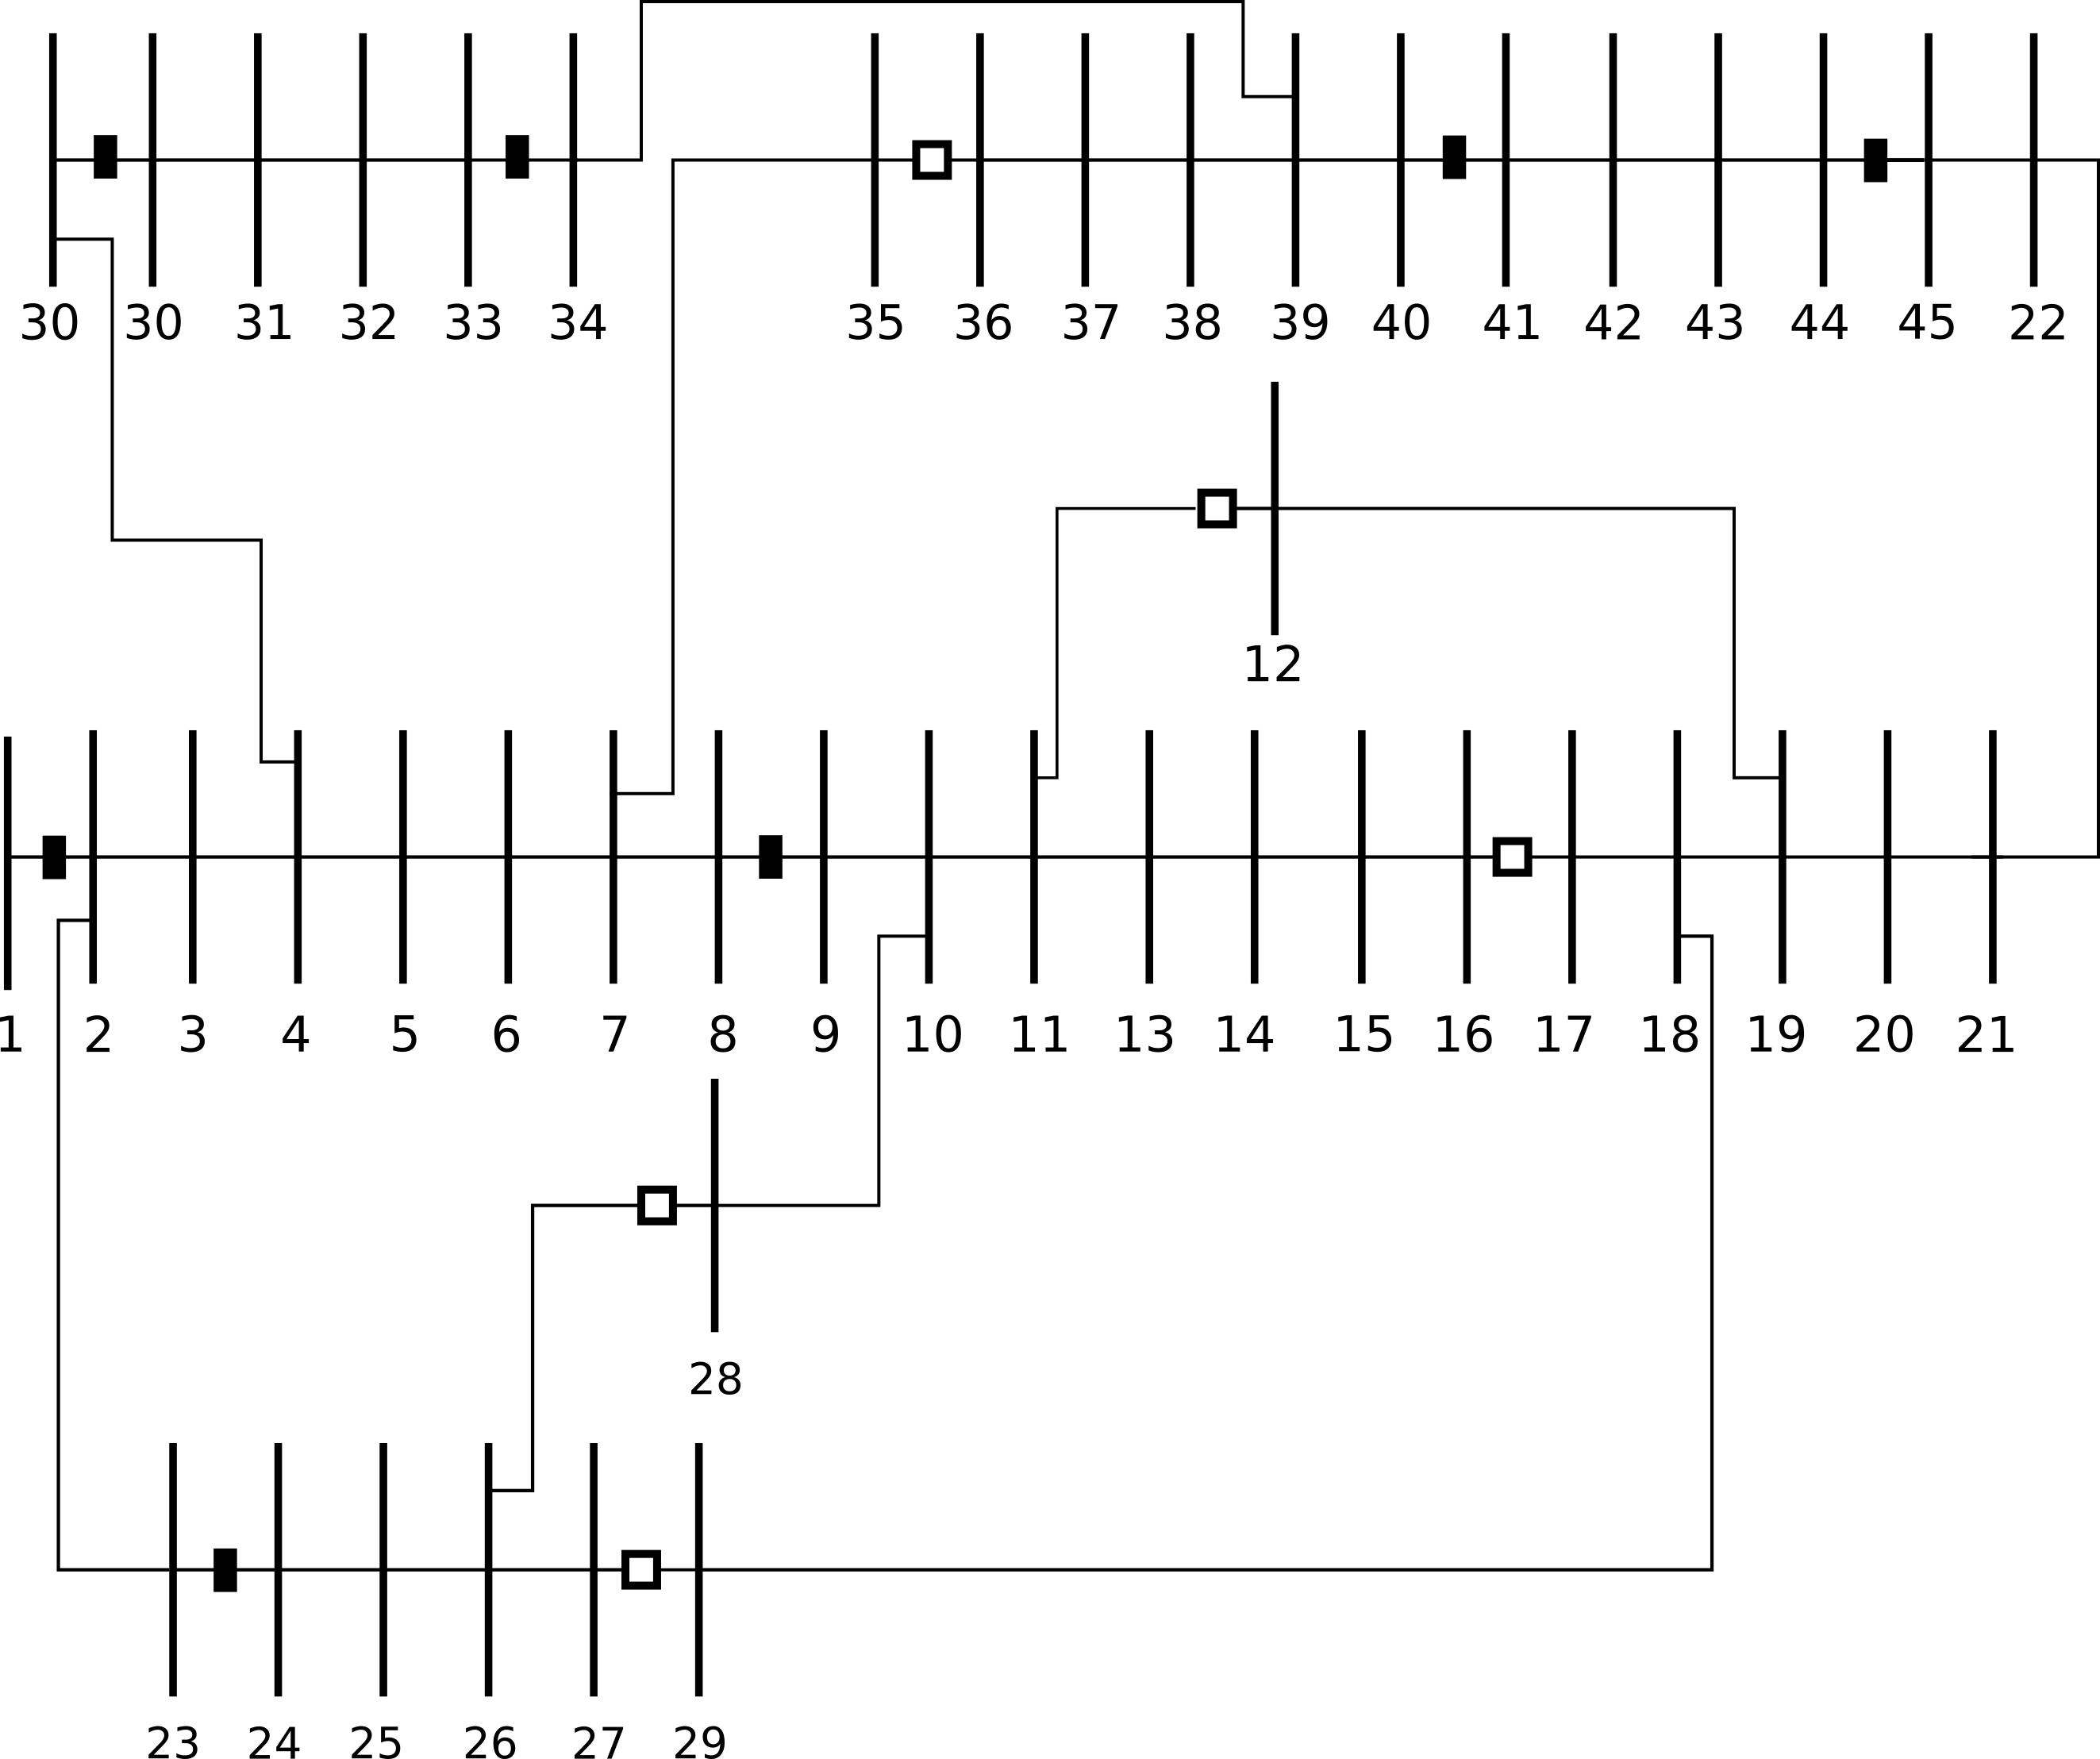
\includegraphics[width=\textwidth]{01_img/rede_otimizada.png}
    \caption{Estado final da rede após a reconfiguração com alimentador no nó 1}
    \label{fig:rede_otim}
\end{figure}

\begin{table}[H]\footnotesize
    \caption{Fluxo de potência ativa entre nós no sistema de 45 nós otimizado}
    \label{tab:fluxo_kw_otim}
    \begin{minipage}{.5\linewidth}
        \centering
        \begin{tabular}{|c|c|c|}
            \hline
            \multicolumn{2}{|c|}{$\Omega_l$} & $P_{ij}$ [kW]  \\ 
            \hline
            2             & 3             & 1256.98                       \\ 
            \hline
            3             & 4             & 1094.83                       \\ 
            \hline
            4             & 5             & 298.27                        \\ 
            \hline
            5             & 6             & 257.82                        \\ 
            \hline
            6             & 7             & 237.02                        \\ 
            \hline
            7             & 8             & 196.89                        \\ 
            \hline
            9             & 10            & 136.65                        \\ 
            \hline
            10            & 11            & 75.60                         \\ 
            \hline
            11            & 13            & 55.01                         \\ 
            \hline
            13            & 14            & 35.00                         \\ 
            \hline
            14            & 15            & 20.00                         \\ 
            \hline
            15            & 16            & 0.00                          \\ 
            \hline
            17            & 18            & -20.00                        \\ 
            \hline
            18            & 19            & -60.05                        \\ 
            \hline
            19            & 20            & -80.14                        \\ 
            \hline
            20            & 21            & -102.65                       \\ 
            \hline
            21            & 22            & -122.85                       \\ 
            \hline
            3             & 23            & 122.09                        \\
            \hline
        \end{tabular}
    \end{minipage}%
    \begin{minipage}{.5\linewidth}
        \centering
        \begin{tabular}{|c|c|c|}
            \hline
            \multicolumn{2}{|c|}{$\Omega_l$} & $P_{ij}$ [kW]  \\ 
            \hline
            24            & 25            & 90.04                         \\ 
            \hline
            25            & 26            & 60.01                         \\ 
            \hline
            26            & 27            & 30.00                         \\ 
            \hline
            4             & 30            & 761.53                        \\ 
            \hline
            31            & 32            & 723.30                        \\ 
            \hline
            32            & 33            & 578.00                        \\ 
            \hline
            7             & 35            & 20.00                         \\ 
            \hline
            36            & 37            & -0.00                         \\ 
            \hline
            37            & 38            & -20.07                        \\ 
            \hline
            38            & 39            & -40.09                        \\ 
            \hline
            39            & 40            & 355.07                        \\ 
            \hline
            41            & 42            & 293.58                        \\ 
            \hline
            42            & 43            & 243.24                        \\ 
            \hline
            43            & 44            & 173.06                        \\ 
            \hline
            10            & 28            & 0.00                          \\ 
            \hline
            12            & 19            & -0.00                         \\ 
            \hline
            18            & 29            & 0.00                          \\ 
            \hline
            22            & 45            & -153.06                       \\
            \hline    
        \end{tabular}
    \end{minipage} 
\end{table}

\begin{table}[H]\footnotesize
    \caption{Fluxo de potência reativa entre nós no sistema de 45 nós otimizado}
    \label{tab:fluxo_kvar_otim}
    \begin{minipage}{.5\linewidth}
        \centering
        \begin{tabular}{|c|c|c|}
            \hline
            \multicolumn{2}{|c|}{$\Omega_l$} & $Q_{ij}$ [kVar]  \\ \hline
             2 &   3 &  495.86\\ \hline
             3 &   4 &  438.82\\ \hline
             4 &   5 &  126.55\\ \hline
             5 &   6 &  111.33\\ \hline
             6 &   7 &  100.63\\ \hline
             7 &   8 &   90.20\\ \hline
             9 &  10 &   60.12\\ \hline
            10 &  11 &   30.05\\ \hline
            11 &  13 &   25.00\\ \hline
            13 &  14 &   20.00\\ \hline
            14 &  15 &   10.00\\ \hline
            15 &  16 &    0.00\\ \hline
            17 &  18 &  -10.01\\ \hline
            18 &  19 &  -25.05\\ \hline
            19 &  20 &  -30.12\\ \hline
            20 &  21 &  -38.46\\ \hline
            21 &  22 &  -43.62\\ \hline
             3 &  23 &   41.89\\ \hline

        \end{tabular}
    \end{minipage}%
    \begin{minipage}{.5\linewidth}
        \centering
        \begin{tabular}{|c|c|c|}
            \hline
            \multicolumn{2}{|c|}{$\Omega_l$} & $Q_{ij}$ [kVAr]  \\ 
            \hline
            24 &  25 &   30.04\\ \hline
            25 &  26 &   20.01\\ \hline
            26 &  27 &   10.00\\ \hline
             4 &  30 &  298.92\\ \hline
            31 &  32 &  282.42\\ \hline
            32 &  33 &  218.27\\ \hline
             7 &  35 &    5.00\\ \hline
            36 &  37 &   -0.00\\ \hline
            37 &  38 &   -5.01\\ \hline
            38 &  39 &  -10.03\\ \hline
            39 &  40 &  130.98\\ \hline
            41 &  42 &   99.50\\ \hline
            42 &  43 &   89.11\\ \hline
            43 &  44 &   58.83\\ \hline
            10 &  28 &    0.00\\ \hline
            12 &  19 &   -0.00\\ \hline
            18 &  29 &    0.00\\ \hline
            22 &  45 &  -53.83\\ \hline
            34 &  39 &  156.59\\ \hline
        \end{tabular}
    \end{minipage} 
\end{table}


  


\begin{table}[H]
    \centering
    \label{tab:pot_chav_otim}
    \caption{Fluxo de potência nas chaves de interconexão do sistema otimizado}
     \subfloat[Fluxo de potência ativa]{
         \centering
         \begin{tabular}{|c|c|c|}
            \hline
            \multicolumn{2}{|c|}{$\Omega_l$} & $P_{ij}$ [kVAr]  \\ 
            \hline
               1 &   2 & 1259.40\\ \hline
               8 &   9 &  136.89\\ \hline
              11 &  12 &    0.00\\ \hline
              16 &  17 &    0.00\\ \hline
              23 &  24 &  122.09\\ \hline
              26 &  28 &    0.00\\ \hline
              27 &  29 &    0.00\\ \hline
              30 &  31 &  731.53\\ \hline
              33 &  34 &  438.00\\ \hline
              35 &  36 &    0.00\\ \hline
              40 &  41 &  295.07\\ \hline
              44 &  45 &  153.06\\ \hline     
         \end{tabular}
     }
     \hspace{3cm} %altera o espaçamento entre as tabelas
     \subfloat[Fluxo de potência reativa]{
         \centering
         \begin{tabular}{|c|c|c|}
            \hline
            \multicolumn{2}{|c|}{$\Omega_l$} & $Q_{ij}$ [kVAr]  \\ 
            \hline
               1 &   2 &  497.09\\ \hline
               8 &   9 &   60.20\\ \hline
              11 &  12 &    0.00\\ \hline
              16 &  17 &    0.00\\ \hline
              23 &  24 &   41.89\\ \hline
              26 &  28 &    0.00\\ \hline
              27 &  29 &    0.00\\ \hline
              30 &  31 &  288.92\\ \hline
              33 &  34 &  158.27\\ \hline
              35 &  36 &    0.00\\ \hline
              40 &  41 &  100.98\\ \hline
              44 &  45 &   53.83\\ \hline
         \end{tabular}
     }
\end{table}

\begin{figure}[H]
    \centering
    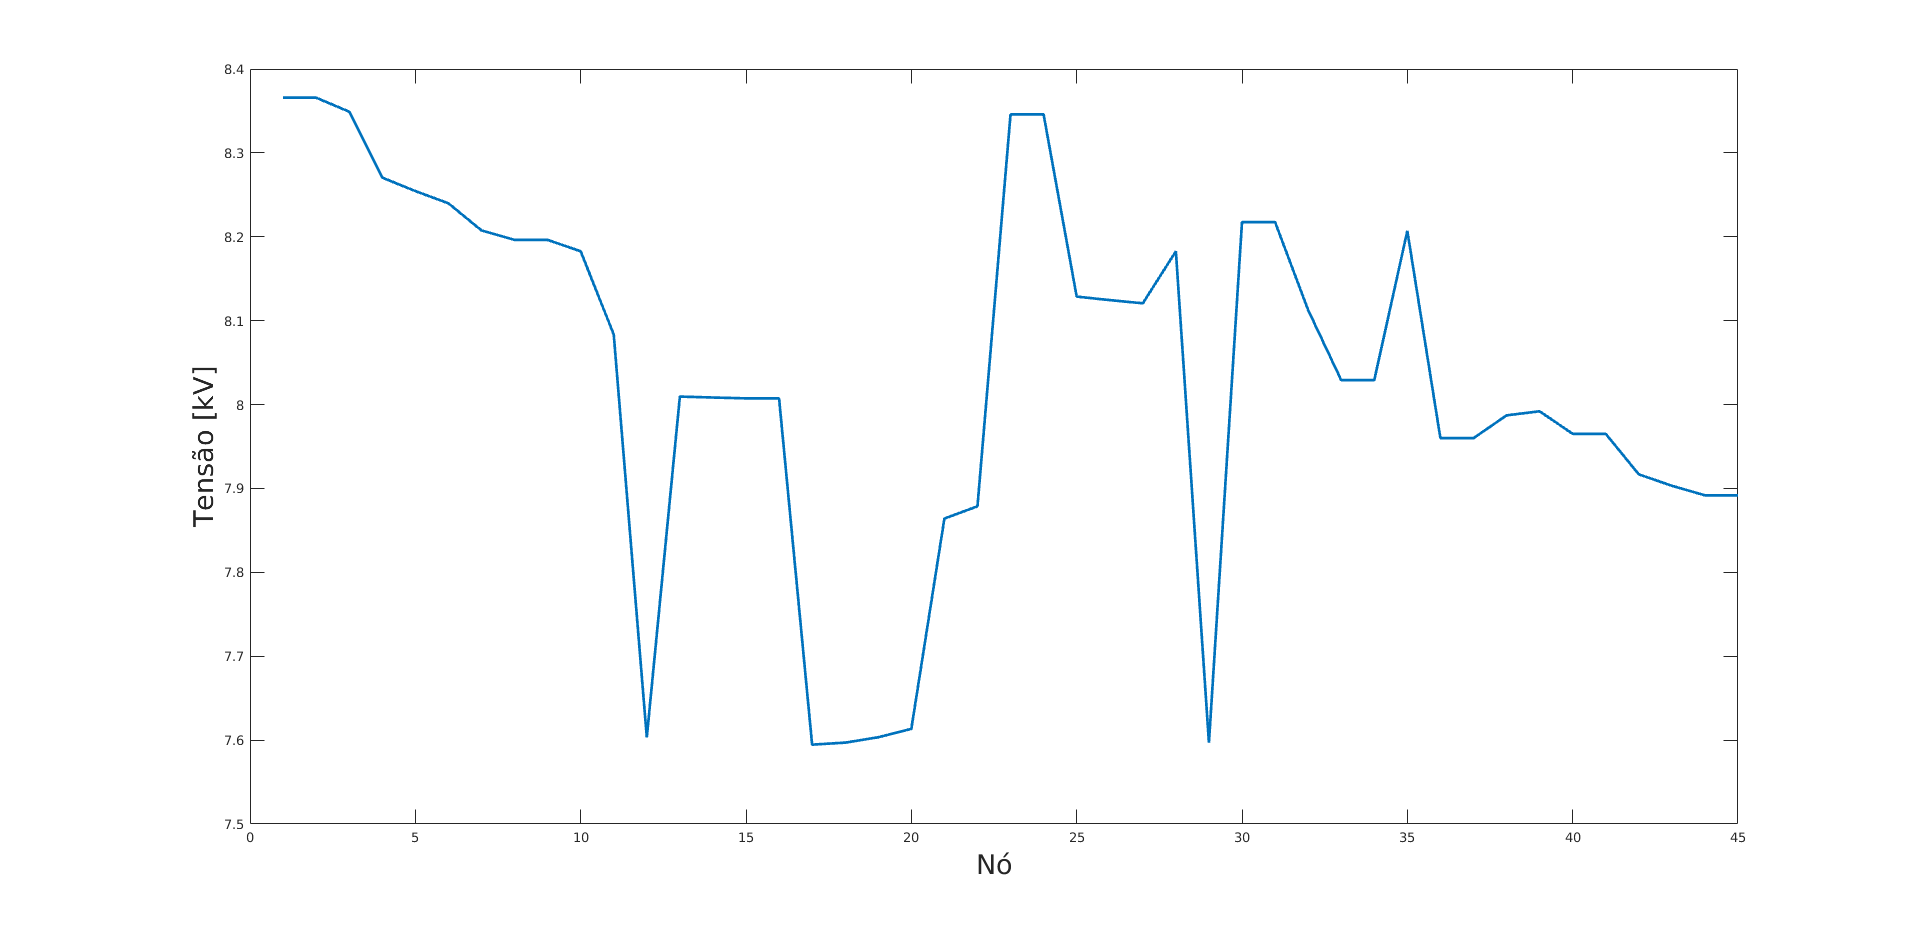
\includegraphics[width=\textwidth]{01_img/Perfil_tensao_otim.png}
    \caption{Perfil de tensão em cada nó após a reconfiguração}
    \label{fig:voltages_otim}
\end{figure}

\begin{table}[H]
    \centering
    \caption{Comparativo operacional entre as duas topologias}
    \label{tab:comp_topologias}
    \begin{tabular}{|c|c|c|}
    \hline
    & Rede Atual & Rede Otimizada\\ \hline
    Perdas de potência ativa [kW]           & 81.50 & 44.39\\ \hline
    Perdas de potência reativa [kVAr]       & 34.65 & 32.08\\ \hline
    Magnitude de tensao minima [kV]         & 6.7982 (0.8532 pu) & 7.5946(0.9532 pu)\\ \hline 
    No da magnitude de tensao minima        & 45 & 17\\ \hline
    Potencia ativa da subestacao [kW]       & 1296.52 & 1259.40\\ \hline
    Potencia reativa da subestacao [kVAr]   & 499.66  & 497.09\\ \hline
    Potencia aparente da subestacao [kVA]   & 1389.47 & 1353.95\\ \hline
    Demanda de potencia ativa [kW]          & 1215.01 & 1215.01\\ \hline 
    Demanda de potencia reativa [kVAr]      & 465.01  & 465.01\\ \hline
    \end{tabular}
\end{table}

\subsection{Discussão dos resultados}

Com base nos resultados observados anteriormente, algumas ressalvas podem ser feitas com relação aos mesmos.

\textbf{citar AgenciaNacionaldeEnergiaEletrica2018ModuloVigencia}
